
\documentclass[10pt, conference,compsoc]{IEEEtran}
\usepackage{hyperref}
\usepackage{graphicx}
\usepackage{cite}
\usepackage[T1]{fontenc}
\usepackage[utf8]{inputenc}
\usepackage{parselines} 
\usepackage{listings}
\usepackage{float}

% *** GRAPHICS RELATED PACKAGES ***
%
\ifCLASSINFOpdf
  % \usepackage[pdftex]{graphicx}
  % declare the path(s) where your graphic files are
  % \graphicspath{{../pdf/}{../jpeg/}}
  % and their extensions so you won't have to specify these with
  % every instance of \includegraphics
  % \DeclareGraphicsExtensions{.pdf,.jpeg,.png}
\else
  % or other class option (dvipsone, dvipdf, if not using dvips). graphicx
  % will default to the driver specified in the system graphics.cfg if no
  % driver is specified.
  % \usepackage[dvips]{graphicx}
  % declare the path(s) where your graphic files are
  % \graphicspath{{../eps/}}
  % and their extensions so you won't have to specify these with
  % every instance of \includegraphics
  % \DeclareGraphicsExtensions{.eps}
\fi
% graphicx was written by David Carlisle and Sebastian Rahtz. It is
% required if you want graphics, photos, etc. graphicx.sty is already
% installed on most LaTeX systems. The latest version and documentation
% can be obtained at: 
% http://www.ctan.org/pkg/graphicx
% Another good source of documentation is "Using Imported Graphics in
% LaTeX2e" by Keith Reckdahl which can be found at:
% http://www.ctan.org/pkg/epslatex
%
% latex, and pdflatex in dvi mode, support graphics in encapsulated
% postscript (.eps) format. pdflatex in pdf mode supports graphics
% in .pdf, .jpeg, .png and .mps (metapost) formats. Users should ensure
% that all non-photo figures use a vector format (.eps, .pdf, .mps) and
% not a bitmapped formats (.jpeg, .png). The IEEE frowns on bitmapped formats
% which can result in "jaggedy"/blurry rendering of lines and letters as
% well as large increases in file sizes.
%
% You can find documentation about the pdfTeX application at:
% http://www.tug.org/applications/pdftex






% correct bad hyphenation here
\hyphenation{op-tical net-works semi-conduc-tor}


\begin{document}
%
% paper title
% Titles are generally capitalized except for words such as a, an, and, as,
% at, but, by, for, in, nor, of, on, or, the, to and up, which are usually
% not capitalized unless they are the first or last word of the title.
% Linebreaks \\ can be used within to get better formatting as desired.
% Do not put math or special symbols in the title.
\title{Aridac: Adaptive Resource Isolation of Non-volatile Devices \\Under  Containerized Environment \\ Project Final Report}


% author names and affiliations
% use a multiple column layout for up to three different
% affiliations
\author{
\IEEEauthorblockN{Xiang Yue}
\IEEEauthorblockA{School of Computer Science\\
Carnegie Mellon University\\
Pittsburgh, Pennsylvania 15213\\
Email: xiangyue@andrew.cmu.edu}
\and
\IEEEauthorblockN{Xuan Peng}
\IEEEauthorblockA{Information Networking Institute\\
Carnegie Mellon University\\
Pittsburgh, Pennsylvania 15213\\
Email: xuanpeng@andrew.cmu.edu}
\and
\IEEEauthorblockN{Zeyu Wang}
\IEEEauthorblockA{Information Networking Institute\\
Carnegie Mellon University\\
Pittsburgh, Pennsylvania 15213\\
Email: zeyuwang@cmu.edu}
}


% use for special paper notices
%\IEEEspecialpapernotice{(Invited Paper)}




% make the title area
\maketitle

% As a general rule, do not put math, special symbols or citations
% in the abstract
\begin{abstract}
Container technology makes cloud computing possible by offering resource isolation and scalability, however, resource sharing brings the problem where heavy containers consume most of the resources and break the fairness. To achieve fairness and maintain a good overall system performance, we propose an adaptive resource isolator for block device namely Aridac, which could adjust the disk resource quota of containers in running time.
\end{abstract}

% no keywords

\IEEEpeerreviewmaketitle

\section{Introduction}
Cloud computing platforms, as a typical instance of infrastructure-as-a-service, nowadays have become the first choice for internet application developers to deploy their services. The main reason behind its popularity is - that cloud computing offers reliability, convenience, isolation, and scalability, along with the pay-as-you-go pricing model. To achieve those features, the quality of service must be ensured with the achievement of resource isolation technologies.\\

Container, as the core part of isolation, creates an illusion for customers as owning the entire system. This lightweight virtualization notion has been widely leveraged by cloud service providers. Based on Linux Cgroup, which offers the ability to isolate resource (e.g. namespace, network I/O, disk I/O), container technologies and applications raised, like Linux Container (LXC) \cite{lxc} and Docker \cite{docker}. Those form the basic units of cloud platforms and are still a great domain for cloud providers to dive deep into. \\

One of the main advantages of adopting containers is "lightweight virtualization". Since each container is just a thin layer around the containerized process, users gain huge efficiencies. However, this lightweight virtualization comes at the cost of sharing the underlying kernel among all containers, and in some cases, this can lead to undesirable effects on resource isolation. The performance of a containerized application heavily depends on which other containers were simultaneously scheduled on the same host. When the cluster scheduler launches new container images on the host, the launching containers may consume too many disk resources. This will cause resource preemption and jeopardize the service stability of existing containers. Therefore, the glaring issue to resolve is resource allocation fairness and preemption avoidance, which means avoiding the resources allocated to containers interfering with each other. For instance, when there are several containers within a node and one of them is running heavy workloads with intense I/O operations, the resources of other nodes can be consumed, greatly delaying the delivery of tasks, like the completion of file reading, the transmission of RPC requests, etc. In addition, Xavier et al. \cite{Xavier2015API} has also analyzed and confirmed the interference of heavy disk workload without limits on resource allocation can degrade the overall performance of the system. Therefore, to avoid sudden delay of container processes, a limitation of resource quota is a good way to control.\\

Although there are already some tools (cgroup, trickle) for adjusting resource quota, the problem is, those tools only offer fixed limitations of resource quota, whereas, in industry, cloud providers can never know how to adjust quota in advance or in real-time - the application in containers and containers themselves are dynamically created, killed and changed frequently. In addition, one of our authors met with the same problem with an intolerant latency of services when resources are consumed mostly by a disk-intensive container. Some works \cite{Sungyong16} manages to alleviate the issue. Since there are still few efforts working on this topic in both academy and industry, our group planned to look into a dynamic way of isolation adjustment.\\

We plan to propose the Aridac, an Adaptive Resource Isolation algorithm of Non-volatile Devices under the heterogeneous containerized environment. The basic idea is to monitor, collect and analyze the resource usage habit of containers as time goes on, and allocate their resources to ensure fairness and preemption avoidance under certain rules. The quota of disk I/O can be allocated by, for instance, the priority of the application, or by containers' history maximum usage. And the objective is to achieve fairness. Besides the algorithm, we plan to design the testing workloads and design experiments for comparing fairness between different policies with specific metrics. Also, we will provide the corresponding benchmark data for further research. To narrow down the scope, we focus on disk isolation, which can be extended to the network I/O or other resource allocation scenarios. The basic tools of system design and experiments include cgroup, bash scripts.\\

The rest of the proposal is organized as follows: the Related Work section shows the relevant works of disk I/O isolation; the Methodology section shows how we analyze the problem and define the basic approach to achieve adaptive quota calculation; Design \& Implementation section includes the system design and engineering implementation of Aridac; the Evaluation section includes Workload Design and Experiment, which we used specific Disk I/O workloads to reproduce the preemption and overload situation, and test whether Aridac could achieve our targeted performance; in the Future Work section, we will discuss few potential improvements on our current approach; in the Problems \& Lessons Learned section we will list few roadblocks we met during the project along with our thinking; in the last section of Conclusion, we will summarize the entire project. \\


\section{Related Works}
Currently, there are not so many efforts on research of container isolation, especially on disk I/O. However, some researchers interested in disk I/O isolation has some works for us to refer. Merchant et al. \cite{Merchant2011MaestroQI} proposed Maestro, focused on the fairness and performance of disk I/O allocation for different applications. He hypothesized there are different performance targets (throughput or I/O directed) for each application, and developed a policy to allocate the resources to them to reach the best overall performance. Arunagiri et al.\cite{Arunagiri2011FAIRIOAA} developed the FAIRIO algorithm to schedule prorated I/O resources for fair allocation, which is a more general solution. Li et al.\cite{Li2015ASCARAC} provided an automatic framework to monitor storage contention and optimize bandwidth utilization. In addtion, for the different scenario on solid state disks, Jo et al.\cite{Jo2017DynamicLB} proposed a I/O load balancer for it. \\

The above ideas give us a good inspiration for container disk I/O isolation. However, those works are not strongly related to our topic. Take Maestro as an instance, it focuses on application I/O balancing on large disk arrays, so its algorithm takes disk I/O ports and preset application targats in consideration with optimization function, which is not aligned with our topic.\\

A naive idea is to treat containers as applications and apply the above solutions. However, different from applications, containers' behaviors are more complicated. In this paper, we believe each container has a dynamic usage pattern and is variable from period to period. Therefore, adjusting the policy to allocate resources cannot be avoided.\\

As for resource isolation tools, Linux control group (cgroup) is the original resource isolation tools, and docker's isolation capacity is built on this. We can easily find the corresonding cgroup of each docker container to limit there resource usage.\\


\section{Methodology}
\begin{figure}
  \centering
    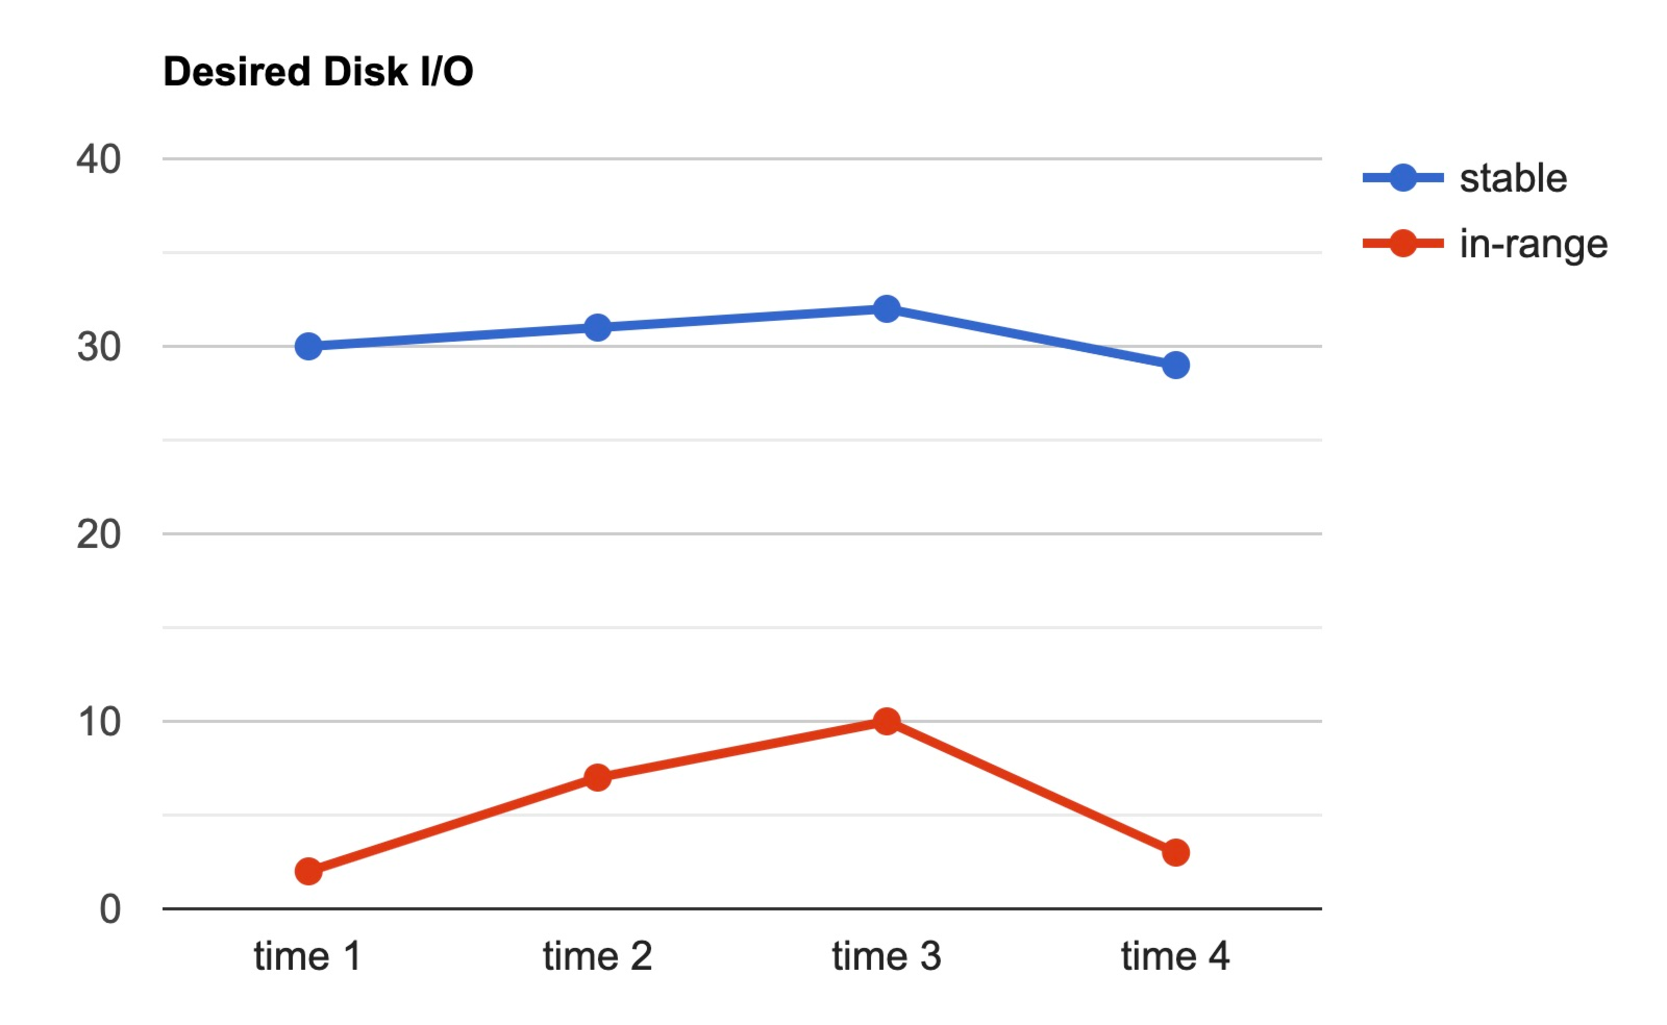
\includegraphics[width=\linewidth]{resources/desired.pdf}
    \caption{desired disk I/O util pattern}
    \label{fig:desired}
  \end{figure}

  \begin{figure}
    \centering
      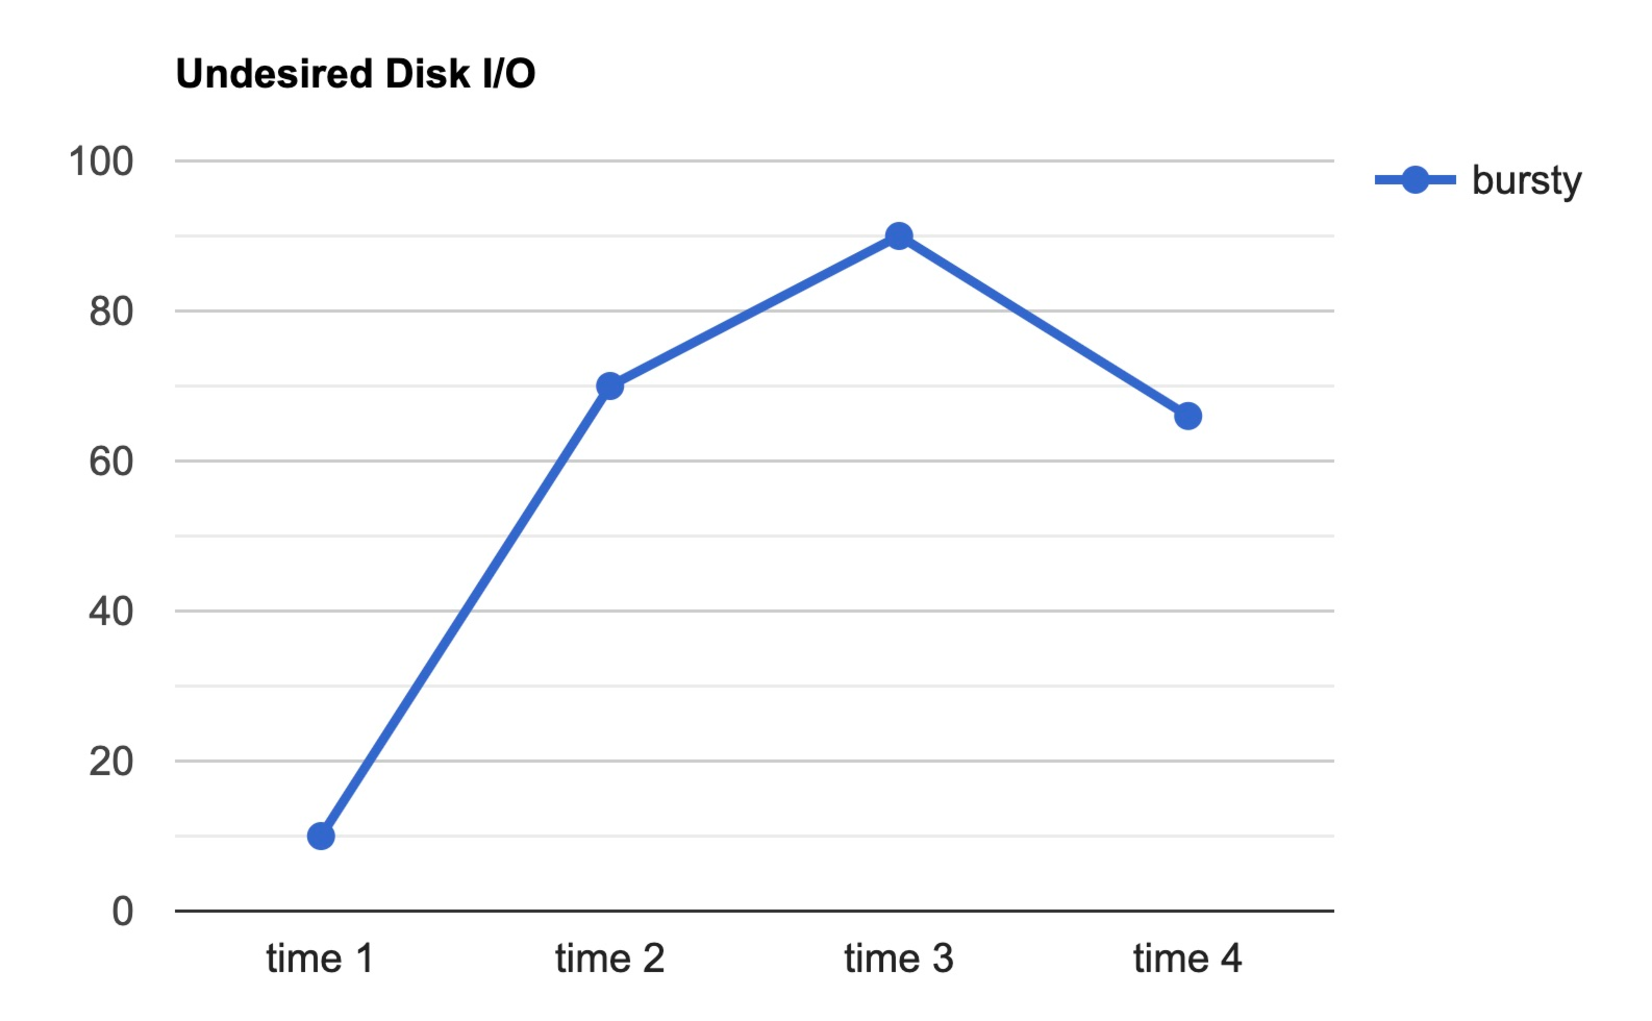
\includegraphics[width=\linewidth]{resources/undesired.pdf}
      \caption{undesired disk I/O util pattern}
      \label{fig:undesired}
    \end{figure}
Can we also take the approach that set a target disk throughput for containers, just as what was done to applications in Maestro? Unfortunately, we can not do the same things with containers, since applications running inside the containers are completely transparent to us. We are not able to know their feature, types, and behavior. We can't even know how many applications would be running in a single container, and how is the target going to fluctuate as the number of containers changes.\\

However, there are still some intuitions that might help with the problem: can we predict the immediately coming disk utilization of a container based on its disk utilization data points in the past period? After a thorough retrospect of the experiences we had with cloud services, we think the answer is yes. In industry, the containers that share a single host machine with others are not supposed to have an unstable and harsh disk utilization pattern. As time goes on, their utilization curves should either remain inside a very stable range, or show some fluctuation at a general low usage level \ref*{fig:desired}. Only under this assumption, these containers can coexist on a single node. For those containers whose guest applications have demanding requirement for disk, such as frequent bursty I/O and high disk utilization \ref*{fig:undesired}, we assert that it's better not to deploy them on a shared machine with any other containers, since it won't be fair for other stake holders. \\

We introduce 2 notion here. The first one is \textbf{lifeline}. If a container shows a stable disk utilization in the past time period, it’s very likely that it needs at least this amount of utilization in order to serve its duty faithfully. We refer this amount of utilization as the lifeline of the container. The second one is abruption. If a container is showing a burst in its I/O utilization, it's very likely due to some abnormal/malicious events. e.g., image downloading, DoS attack. We refer this kind of traffic pattern as abruption. To summarize, we hold the view that lifeline deserves higher priority than abruption! \\

So for those containers with stable disk utilization pattern, we can gather  their historic data points, and then do some aggregation to estimate their lifelines. The aggregation is not necessarily supposed to be sophisticated. Simple and straightforward operatio, such as average, should be able to serve as a good-enough lifeline estimation. \\

On top of the estimated lifelines, we can experiment and apply various isolation policy. For the firstly isolation policy in this initial version of Aridac, we introduce an elastic ratio \textit{P}. We assert the next-round utilization will be in the range of up to \textit{lifeline*(1+P)}. And this is value, \textit{lifeline*(1+P)}, will be set as the cap of disk utilization in the coming round for a container.\\

\section{Design \& Implementation}
\begin{figure}
  \centering
    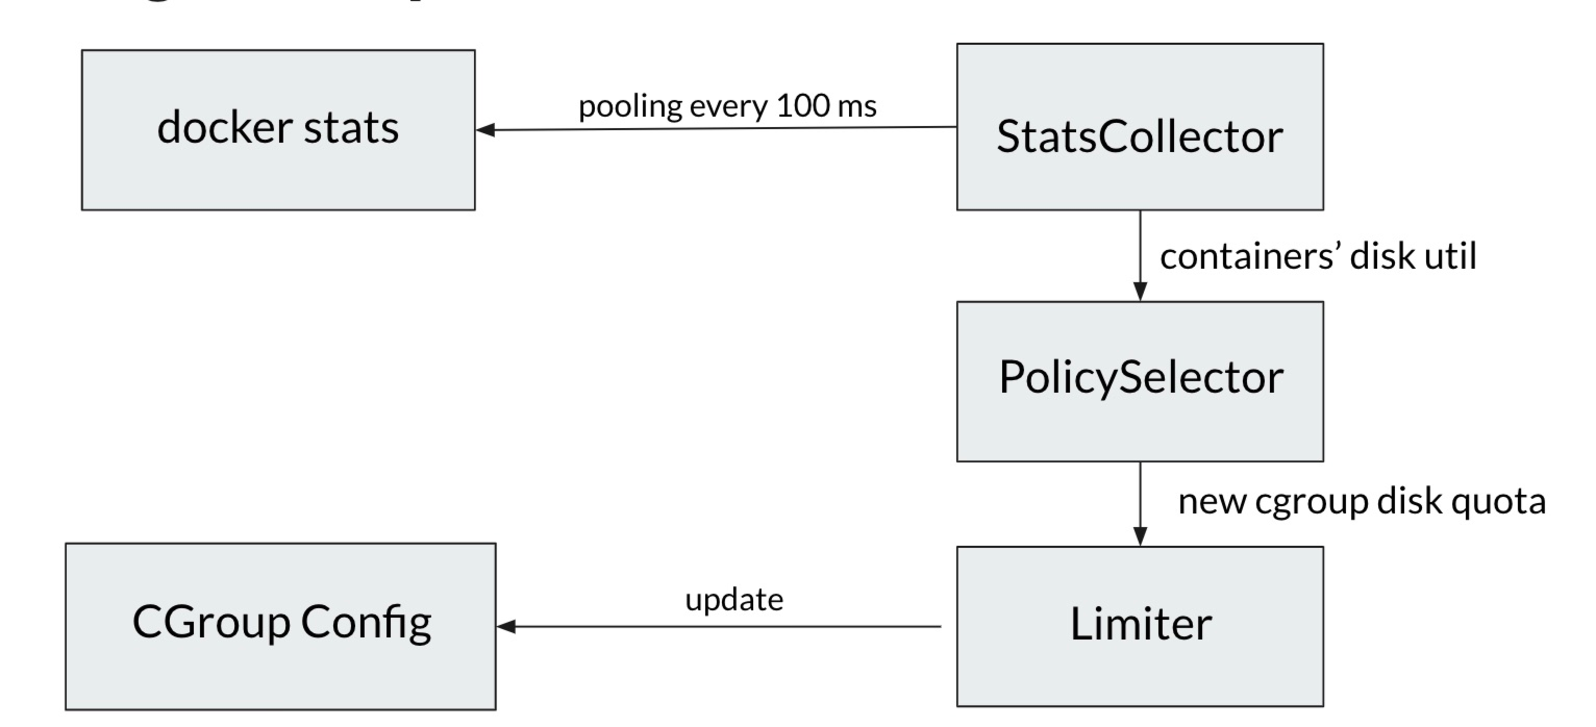
\includegraphics[width=\linewidth]{resources/design.pdf}
    \caption{system overview}
    \label{fig:design}
  \end{figure}
We present the design \ref{fig:design} and implementation overview of Aridac in the coming paragraphs. \\

\subsection{Stats Collector}
The architecture of Aridac is pipelined. First, Aridac depends on the Docker native stats command \textit{docker stats} in order to get the disk throughput of container. The disk throughout shown by docker stats is the accumulative disk throughout since the start of a container. So we subtract the previous throughput on the latest one to get the delta value. And this delta value is the amount of disk throughput that's been done between the last 2 sampling points. Since the interval of the refreshing of the output stream of docker stats is somewhat varying, the StatsCollector of Aridac will keep polling the output stream of docker stats command at a fixed interval that is a lot smaller than the one of the output stream in order to process the latest data in a timely manner. The StatsCollector also record the timestamp of its last receiving refresh from the output stream, so that we can calculate the disk throughput per unit time. And disk throughput per unit time will be used to calculate the disk utilization rate of a container.At the end of StatCollector, we get the disk utilization rate of every living container. We will push the rate to a bounded queue with a fixed length of N. This queue is the output of StatsCollector and also the input PolicySelector.\\

\subsection{Policy Selector}
Once the execution enters PolicySelector, we then do various aggregation to the collected data and select the isolation policy we want to apply. In the initial version, we implemented the simple aggregation that takes the average of all these history utilization rates inside the bounded queue. And the average value we get is the lifeline. And the policy we use is to set a cap disk utilization value \textit{lifeline*(1+P)} for each individual container.The current implementation the \textit{P} we use is 20\%. \\

And after having all the caps calculated, we check if the sum of the cap is bigger than 1. If so, it shows the disk contention is pretty intense and the system enters a unstable state, where disk utlization may quickly reach 100\% and the performance of guest applications could be severely jeopardized. So in this case, we will prompt alert to the user or system admin just so to let them be aware of the resource shortage, so that they can take measures like redeploying some containers in another machine, or add more disks to ease th situation. An interesting improvement we can do here, is to implement an auto disk scaling mechanism. With the help of an auto tool, the redeployment and scaling of the disk can be triggered without the intervention of any human resource. And the tool can also be more responsive to problems than human can be.\\


\subsection{Limiter}
Limiter is the abstraction of Linux cgroup resource control mechanism. There are several interfaces provided in the limiter, which are used to set the cap of disk input and disk output rate for any specific process. In the PolicySelector, after we have calculated the caps, we then call the interface in limiter to actually send the command to the system, by writing our new caps into the config file of each individual cgroup. For docker containers, each one of them has its own cgroup, whose config file can be indexed with the container id. So it's very convenient for us to set the caps in Limiter.


\section{Evaluation}

In this section, we aim to prove two major things. First, the scenario of resource preemption exist; second, to test if our policy is able to prevent the resource preemption, and the quota limit can adapt the dynamic desire of application (e.g. increase or decrease). To achieve the measurement of the correctness and performance of the Aridac, we proposed two workloads to reproduce the typical disk bandwidth preemption problem and resource overloading problem, and see how would Aridac achieve better resource isolation on those two workloads.

\subsection{Workload Design}
For the first workload, we want to reproduce the situation where one victim container runs stably on its lifeline, while the other burst container rapidly grows and starts to obtain the disk bandwidth of the victim container for a long period of time. We want to use this workload to simulate the case that one of the containers starts to require much more disk bandwidth for its long-run job, and it is possible to exceed the maximum Disk I/O rate and cause the system to enter an unhealthy state.

\begin{itemize}
  \item \textbf{Workload 1} Two containers A and B running with same rate (200KiB/s) in the beginning. At some point, B's I/O usage goes high without limit (2MiB/s), preempting A's resource.
\end{itemize}

For the second workload, we want to reproduce the situation where one victim container runs stably on its lifeline, while the other burst container rapidly grows and starts to obtain the disk bandwidth of the victim container for a short period of time, and then its disk I/O rate will drop to the stable state. We want to use this workload to simulate the case that a new container launched on the physical node, the burst disk I/O is caused by the container initialization process.

\begin{itemize}
  \item \textbf{Workload 2} Two containers A and B running with same rate (200KiB/s) in the beginning. At some point, B's I/O usage goes high without limit (2MiB/s), preempting A's resource. After a while, B's usage goes back to normal rate (200KiB/s).
\end{itemize}

Our policy should prevent the above resource preemption. Also, the quota allocated by our policy should keep align with the containers' desire dynamically. The only difference between two workloads is that, in workload 2, B's usage goes back to its normal rate, where our policy should be able to adjust the quota low. 

\subsection{Experiment}
To measure the correctness and performance of Aridac, we performed each workload twice, the first time without any resource isolation policy, and the second time with our Aridac Adaptive Policy. The experiment is set on a PDL Narwhal bare metal machine with 75 GB of hard disk, the environment {MAX\_DISK\_IO} is set to 1 MB/s, which means the resource allocation policy is calculated base on allocate total of 1MB of bandwidth to the two containers.\\

To measure the correctness and performance of Aridac, we performed each workload twice, the first time without any resource isolation policy, and the second time with our Aridac Adaptive Policy. The experiment is set on a PDL bare metal machine with 75 GB of hard disk, the environment MAX\_DISK\_IO is set to 1 MB/s, which means the resource allocation policy is calculated base on allocate total of 1MB of bandwidth to the two containers.\\

\begin{figure}[h]
\centering
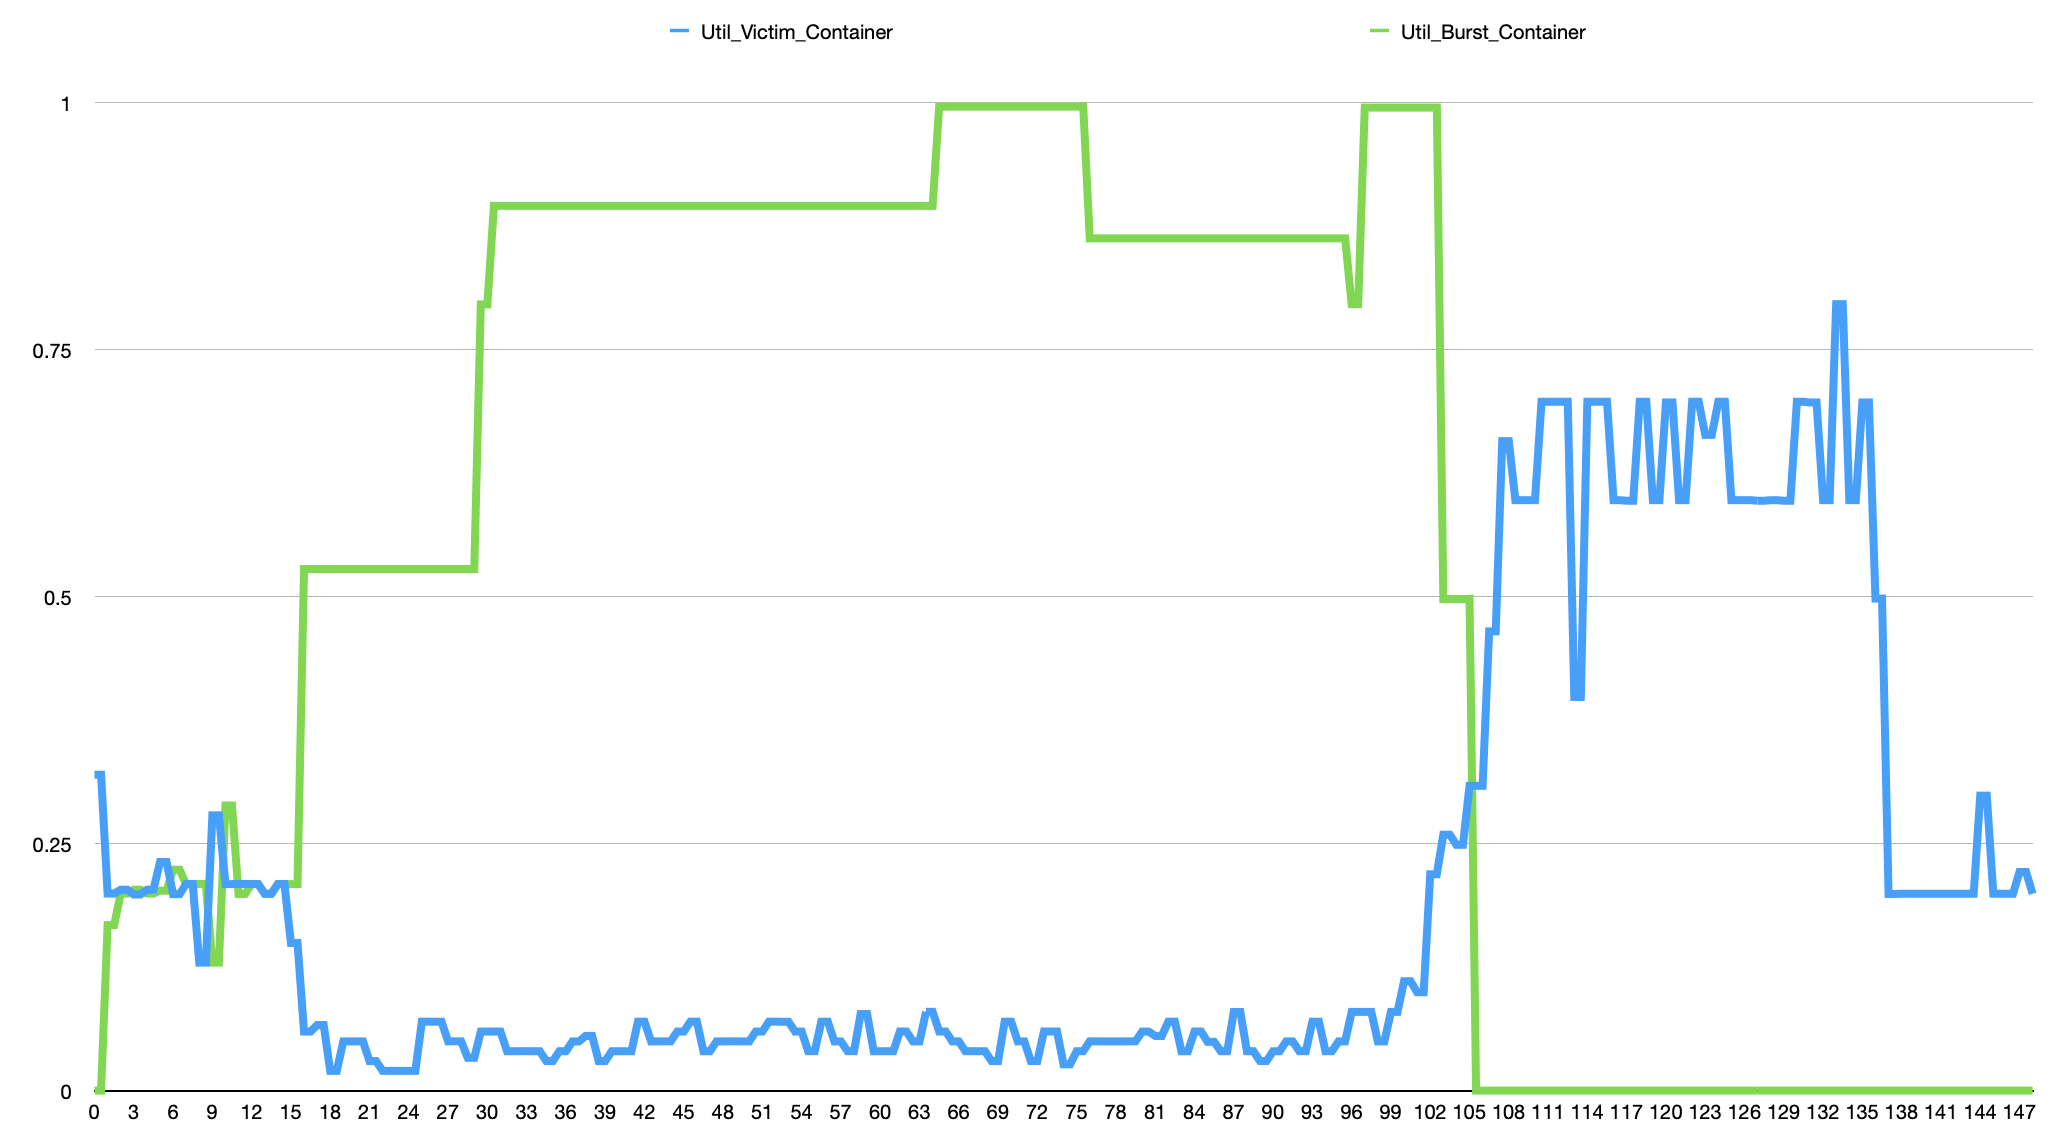
\includegraphics[width=0.5\textwidth]{images/workload1_1.png}
\caption{Workload 1 Running Without Any Policy}
\end{figure}


Figure 4 demonstrated the situation of workload 1 running without any resource limitation policy, the figure is measured by the overall disk bandwidth utility for each container over time. As the figure shows, in the beginning, both two containers are generating disk IO at a stable rate of about 200 KB per second. After about the 15th second of launching the workload, the burst container starts to generate a large amount of disk IO, which results in obvious bandwidth preemption on the victim container. The actual disk IO utility rate of the victim container dropped to nearly 0 from the 15th second through the 105th second. In this workload, we are actually to demonstrate the case in which the burst container keeps running on the high disk IO generate rate, but we still limited the total running time of the burst container, to allow the metrics to display the delayed disk IO in the queue. At the 105th second, the workload stopped the burst container, and the figure shows the disk IO rate of the victim container increased quickly. Since the victim container is still generating IO workload at 200 KBps, the additional bandwidth taken by it is actually performing its delayed IO volume in the queue. This is the exact unhealthy state we are trying to avoid.\\

\begin{figure}[h]
\centering
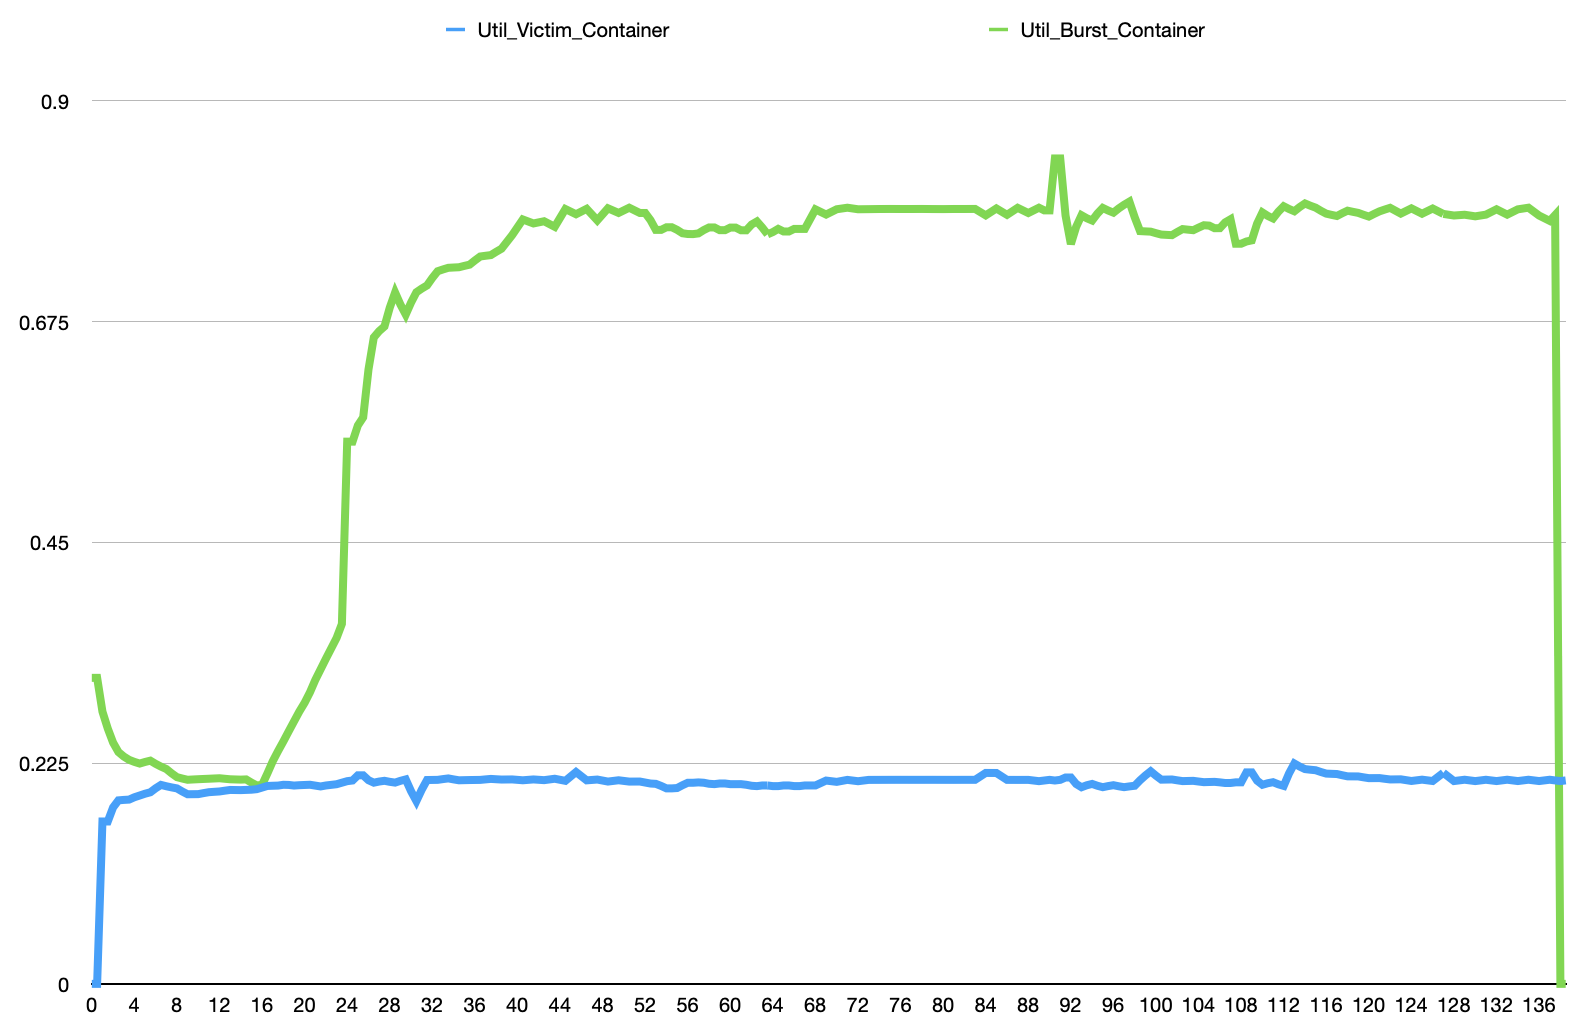
\includegraphics[width=0.5\textwidth]{./images/workload1_2.png}
\caption{Workload 1 Running With Aridac}
\end{figure}


Figure 5 demonstrated the situation of workload 1 running with our Aridac Adaptive policy, the figure is measured by the overall disk bandwidth utility for each container over time. Similar to figure 4, in the beginning, both two containers are generating disk IO at a stable rate of about 200 KB per second. After about the 15th second of launching the workload, the burst container starts to generate a large amount of disk IO, but the preemption is avoided with Aridac. The actual disk IO utility rate of the victim container consistently stayed at its desired rate to maintain its lifeline, while the burst container gained idle bandwidth exponentially. As we limited the total running time of the burst container, the accumulated disk IO volume is the same as in the case in figure 2.  Therefore we can see that while the Aridac kept the bandwidth of the victim container uninvaded, the burst container can still consume as much as the remaining bandwidth it needs to accelerate its workload. It finished the same amount of disk IO at the 136th second instead of the 105th second, and during the entire process, the victim container remains healthy and is able to provide stable services.\\

\begin{figure}[h]
\centering
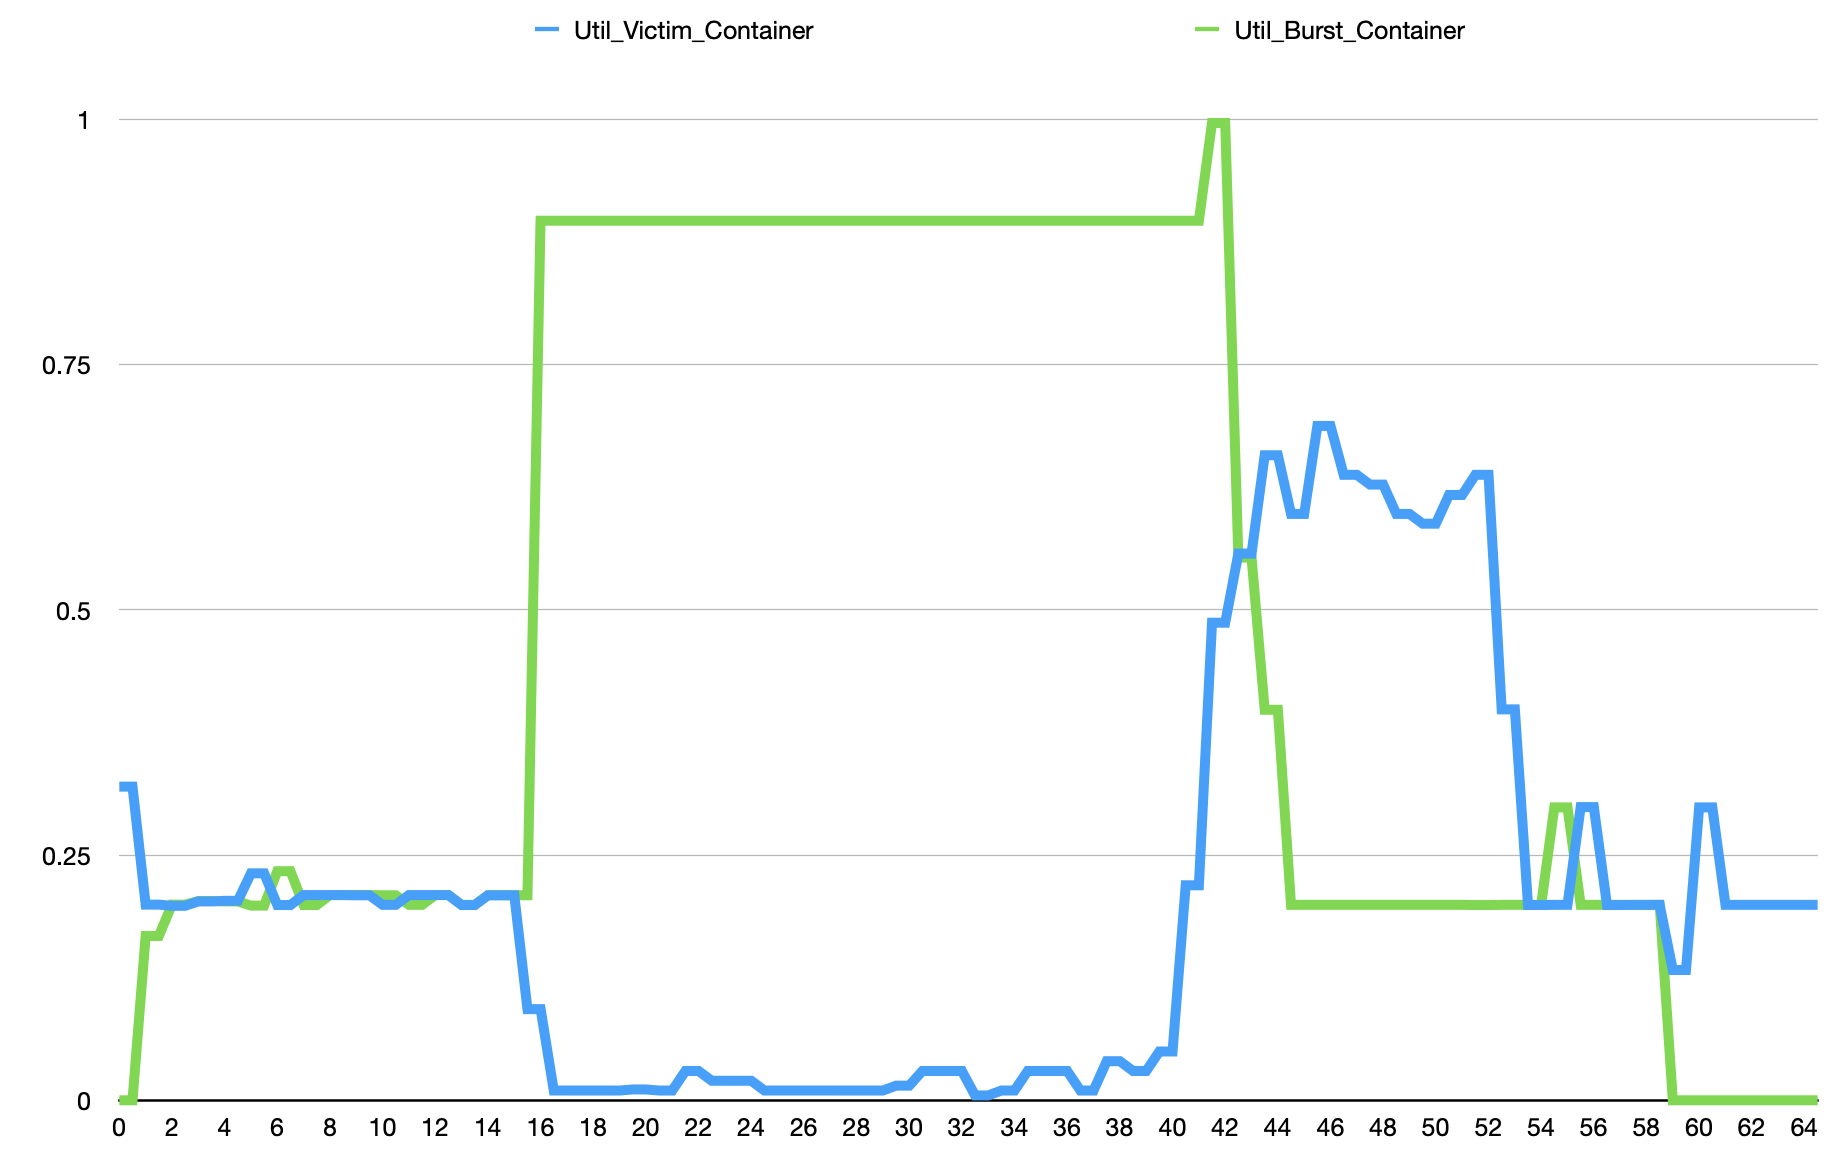
\includegraphics[width=0.5\textwidth]{images/workload2_1.png}
\caption{Workload 2 Running Without Limitation Policy}
\end{figure}


Figure 6 demonstrated the situation of workload 2 running without any resource limitation policy, the figure is measured by the overall disk bandwidth utility for each container over time. The overall design of workload 2 is very similar to workload 1 we just introduced, besides it only produces a large amount of disk IO for a relatively short period and will eventually drop to a relatively low but stable rate to maintain its lifeline. As the figure shows, in the beginning, both two containers are generating disk IO at a stable rate of about 200 KB per second. After about the 15th second, the burst container starts to generate a large amount of disk IO and starts to preempt disk bandwidth on the victim container. The actual disk IO utility rate of the victim container dropped to nearly 0 from the 15th second through the 40th second. At the 40th second, the workload of the burst container dropped to its long-run stable rate, and the figure shows the disk IO utility of the victim container increased quickly due to accumulated delayed IO volume in the queue. The system is in an unhealthy state.\\

\begin{figure}[h]
\centering
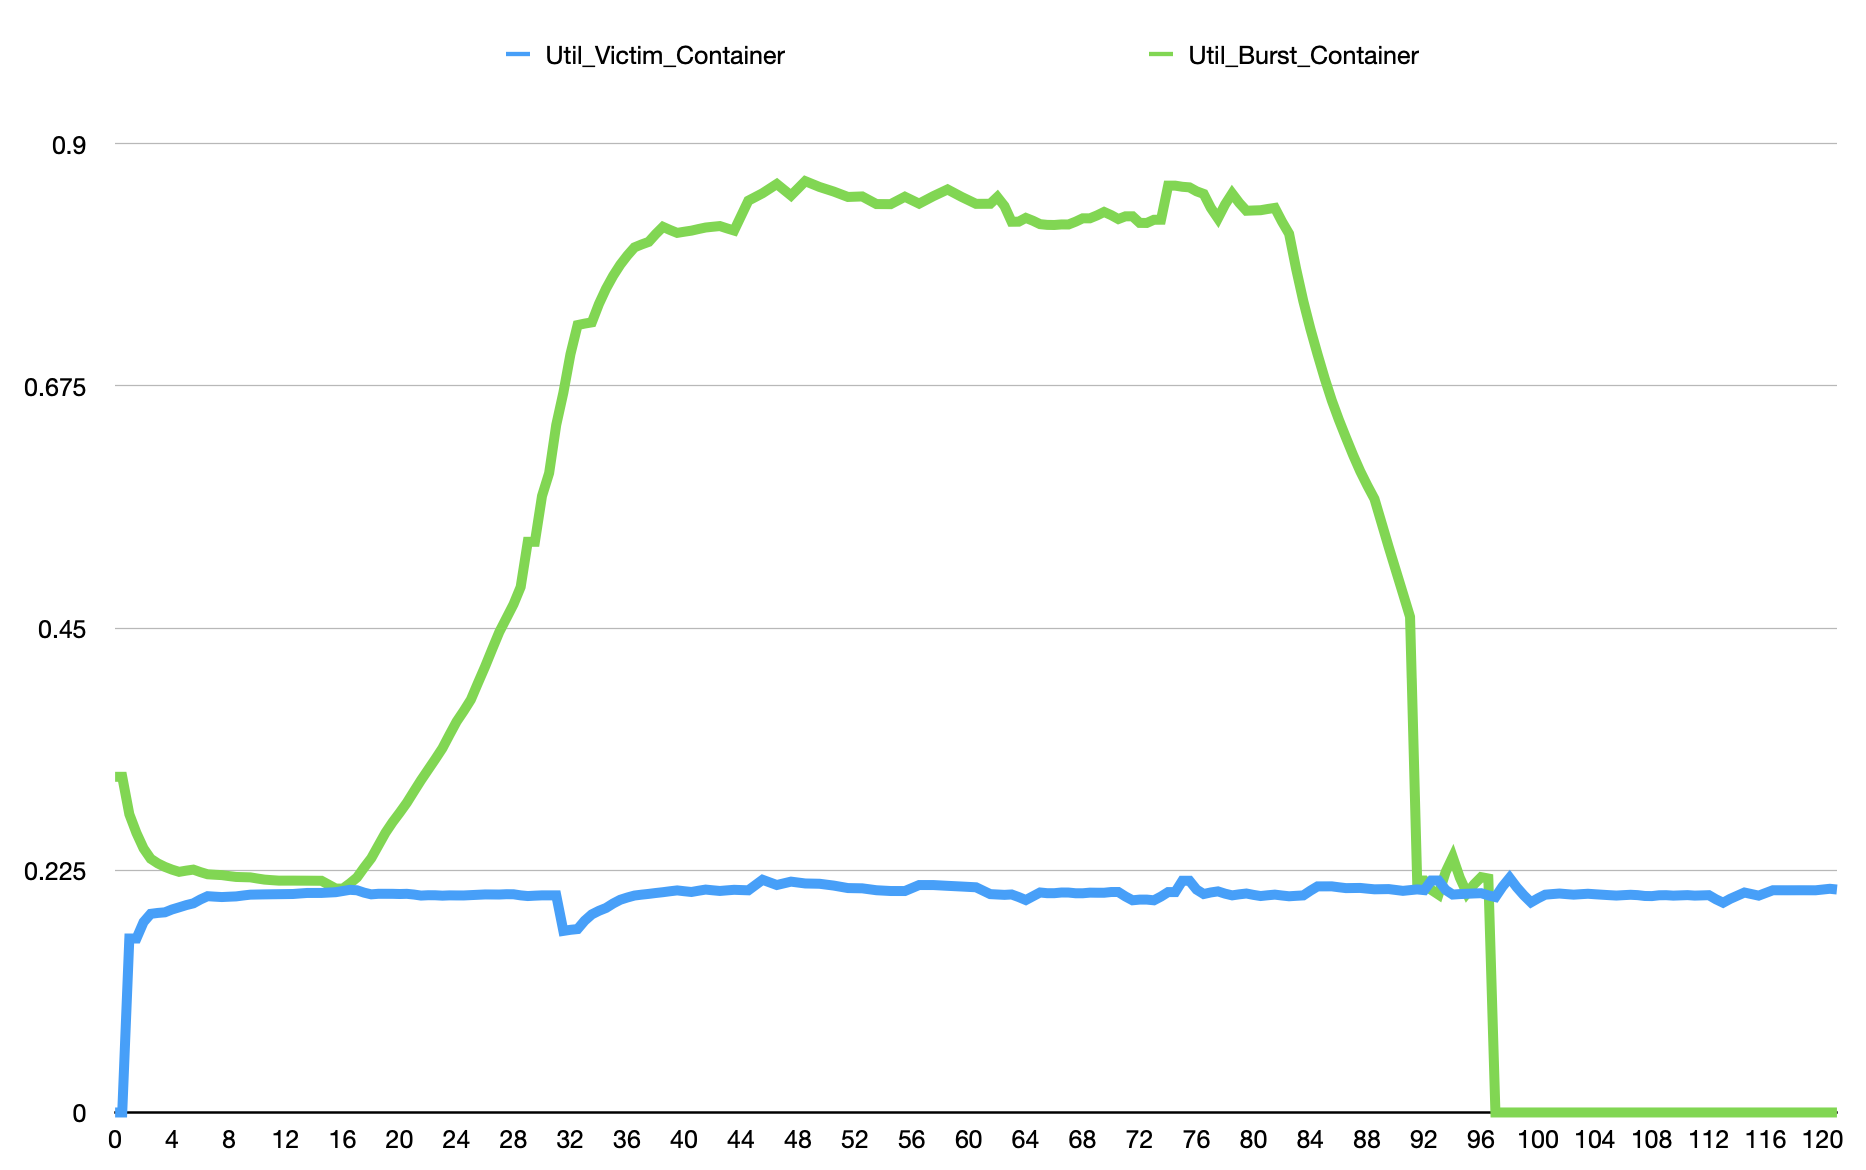
\includegraphics[width=0.5\textwidth]{images/workload2_2.png}
\caption{Workload 2 Running With Aridac}
\end{figure}

Figure 7 demonstrated the situation of workload 2 running with our Aridac Adaptive policy, the figure is measured by the overall disk bandwidth utility for each container over time. Similar to the previous figures, in the beginning, both two containers are generating disk IO at a stable rate of about 200 KB per second. After about the 15th second of launching the workload, the burst container starts to generate a large amount of disk IO, but the preemption is avoided with Aridac. The actual disk IO utility rate of the victim container consistently stayed at its desired rate to maintain its lifeline, while the burst container gained idle bandwidth exponentially. Aridac only responds quickly to the burst container, and it only takes about 10 seconds to allocate all idle bandwidth to the burst container step by step. While the burst workload finished and returned to the stable rate at the 80th second, Aridac was able to reclaim the bandwidth previously allocated to the burst container based on the change in disk IO rate is observed. During the entire process, the victim container remains healthy and is able to provide stable services, and all the idle resources are well managed based on the on-demand policy.\\

Therefore, with Aridac tracking and managing the disk IO bandwidth on the node, we were able to avoid squeezing the lifeline of the victim container for both workloads. In the first workload, as we proposed the overloaded state on the physical node will continue for a long period of time due to the burst container continually generating disk IO at a rate beyond what the system could handle, Aridac is also functional to provide warning notifications to let the administrator be awarded that the system is overloaded. Then the owner of the container will be able to decide to terminate one of the containers or migrate the services to a more suitable location. Thus, the behavior of Aridac is aligned with our expectation.\\




% conference papers do not normally have an appendix

\section{Conclusion}
We conducted a thorough investigation about the problems existed for disk contention under modern containerized environment. We found out that the disk resource isolation level among containers is not good enough to ensure a consisten behavior pattern and perfornmance of the whole system. On a shared physical node where multiple containers are running stably, disk contention \& preemption may occur due to unexpected events.\\

We further did our literature review in search of disk utilization quota control relevant topics. And the work we found served as good insights, but cannot be directly applied to our problem because of the difference in domain. \\

We figured out the historic disk utilization statistics may be useful in predicting the incoming short-term disk utilization. And we followed this hypothesis and implemented Aridac, with a pipelined system architecture which includes 3 phases namely StatsCollector, PolicySelector, and Limiter. We futher show that Aridac achieved the desired adaptive disk resource isolation capability under the simulated environment with several carefully-designed workloads.\\

To conclude, with Aridac, we are able to adjust the resource cap for each container adaptively, so that programs in the guest containers could maintain a consistent performence throughout their lifetime.

\section{Problems Encountered}
We encountered many troubles throughout the whole journey. For example, we were disturbed by not being able to reproduce the case where a container with high disk I/O could preempt the disk share of the other container. Also, at the beginning stage of the evaluation, we planned to use Death Star microservice benchmark as the testbed. But later we found that the launching of Death Start will cause a lot of dependency issues and mess up the test environment. And the other time-consuming task is to find the suitable disk I/O generator. We tried different kinds of approach, from self-improvised C program, to the dd shell command, and finally the fio. And the usage of fio is a bit complex, with a lot of available arguments and options. Fortunately the documentation is very helpful, and we were able to find everything we want from it.\\

\section{Future Work}
Although the current implementation of Aridac already meets our initial goals, we believe there are still multiple directions to improve the project. Most of the ideas are focusing on improving the usability of Aridac so we can deploy it in the real-world environments.\\

The first idea is to enable Auto MAX\_DISK\_IO Probing. As we mentioned in the earlier part of the paper, Aridac uses a global variable MAX\_DISK\_IO to calculate the disk IO resource limitation, which is currently manually configured and immutable during the experiment. The design of the system requires the MAX\_DISK\_IO as much as accurate to achieve the best resource allocation accuracy. As we know the hardware is not always running stably, especially for hard disks, which can be easily affected by humidity, temperature, and vibrations on the rack. The current fixed setting is good enough for a very short test workload, but will definitely perform much inefficiently in a real-life long-run environment. As we tested the current version of Aridac on a more complex workload in which two containers generate burst loads in turns, we observed a preemption happens due to actual MAX\_DISK\_IO rate decrease.

\begin{figure}[h]
\centering
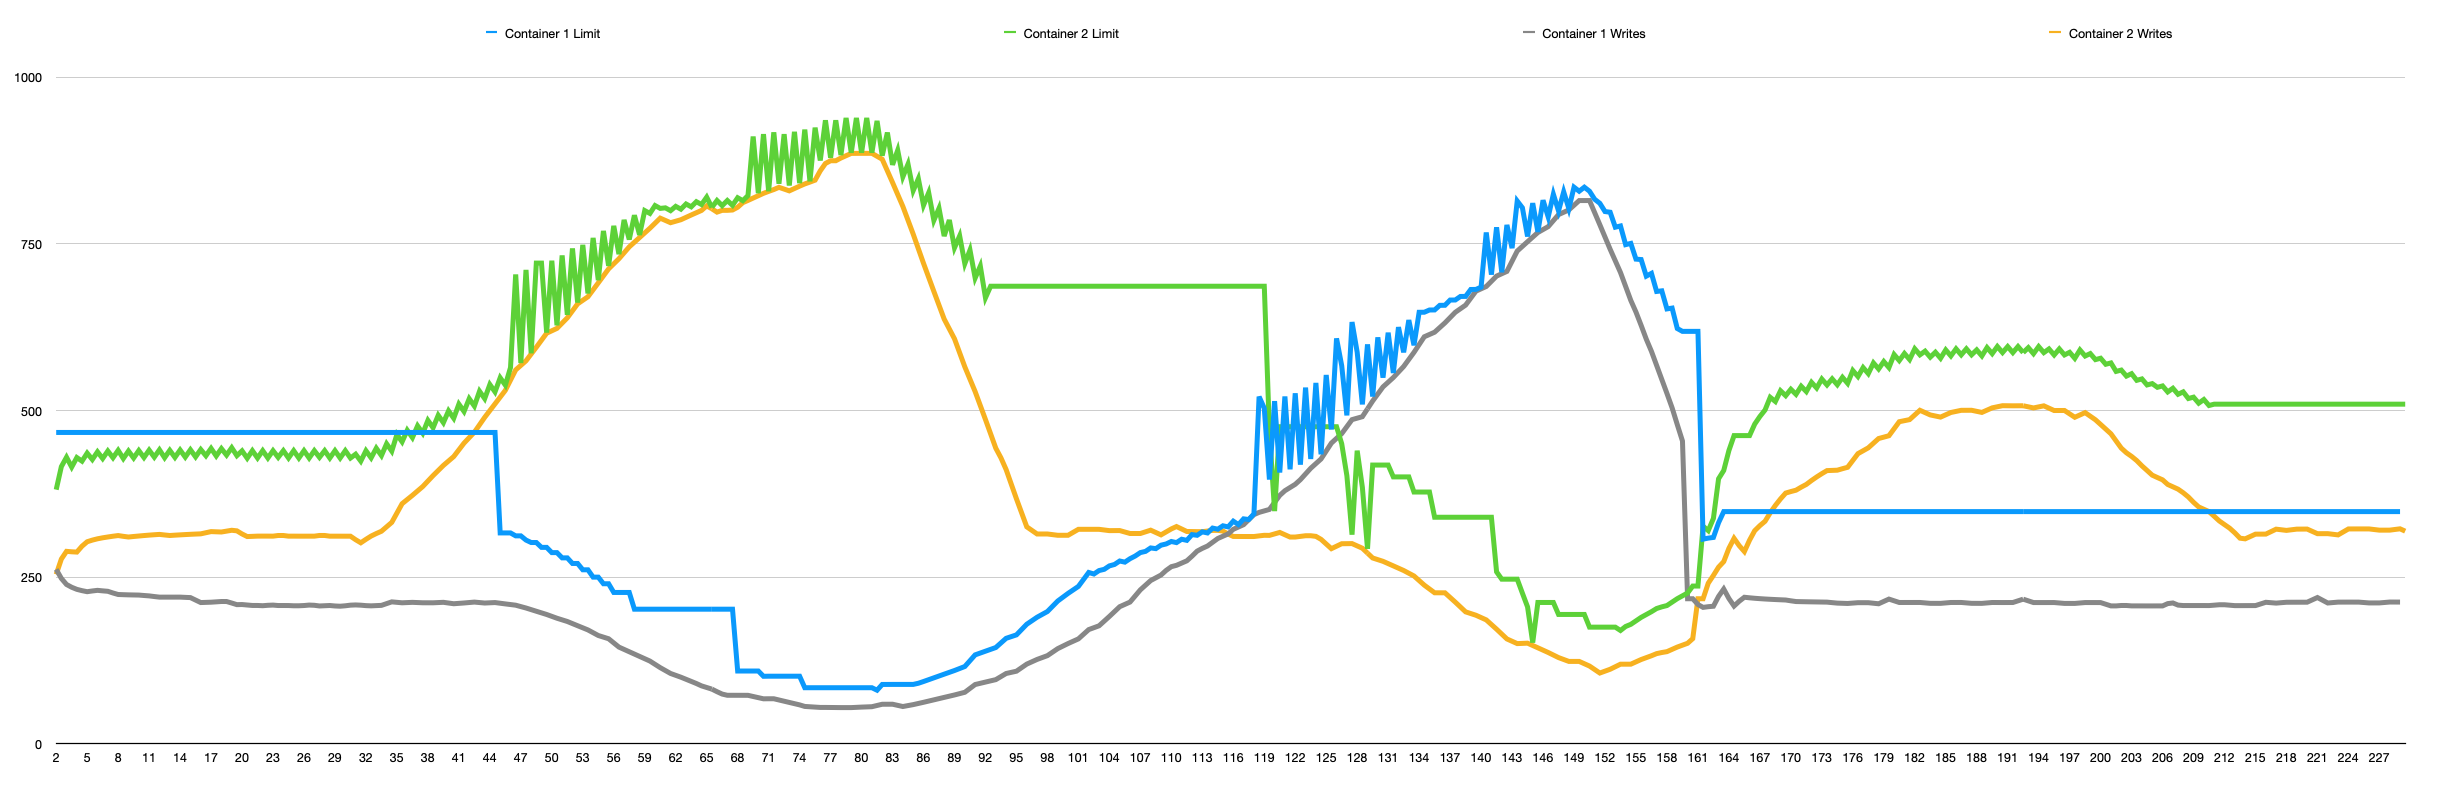
\includegraphics[width=0.5\textwidth]{images/workload3.png}
\caption{Repeating Waves In Turns}
\end{figure}

In figure 8, we use the actual disk IO rate on Kb per second instead of disk utility to measure the demonstrate the change of disk IO for each container along with their adaptive quota. We can find the preemption happened after the 50th seconds. As the blue line displayed that the assigned quota to container 2 is not well used, a scale-in occurs right after it and caused the preemption. The fact is the quota is calculated based on the fixed MAX\_DISK\_IO variable of 1 MB per second, as the actual MAX\_DISK\_IO dropped, container 2 will not obtain the promised amount of bandwidth. Since Aridac is using the historical metrics to determine the desired resource for each container, it can not tell if the historical IO rate changes due to MAX\_DISK\_IO changes or the containers actively reduce their desired bandwidth. So the inaccurate measurement of MAX\_DISK\_IO can lead to undesired quota updates which reduce the resources allocated to a container and lead to unhealthy states.\\

The simplest way to obtain the real-time value of MAX\_DISK\_IO is to run an IO test directly on the disk, but it will consume unnecessary resources in a long-run program. One way to implement the Auto Probing is to use a ballooning like approach, maintaining a driver running outside of the container groups with lowest priority on disk I/O. Thus it will consume and measure any idle disk bandwidth in the system if the actual MAX\_DISK\_IO is higher than our configuration; in the other case, it will decrease to 0 if the actual disk MAX\_DISK\_IO is running below our configuration.\\

Another improvement we considering implementing is to support multiple disks on a single node. The current stats implementation relies on the docker stats command, which does not support volume counts on separate disks. Thus, we will not be able to support any bandwidth allocation for a multi-disk physical node. This improvement can take a lot of work to finish, we will probably need to implement our own stats functionality at the bottom of the Linux kernel. But it can be an important demand if we want to deploy Aridac in the real-world environment since multi-disk storage is very common on disk-heavy clusters.\\

The third improvement is to implement a more complex allocation policy to achieve fairness for containers with different assigned priorities. Our current scenarios do not include any preassigned priorities, which is ideal for simple policy but not close to the industrial use cases. We may also provide a much more flexible policy for the user to configure the Aridac policy more than the current case of the single configuration on ELASTIC.\\

The last idea will be to extend the warning notification functionality to horizontal disk auto-scaling. As a new trend, the public cloud providers now started to offer products that are elastic in defaults, which means the user can scale out existing instances without relaunching or migration. In some research\cite{park2020more}, the author explored the possibility of auto-configure disk settings on the public cloud with the simple input of desired performance on bps or IOPS. This action can be adopted as an extension of the warning notifications functionality to cure unhealthy nodes by purchasing more resources on the public cloud. Therefore, Aridac will also release the user from the overload problem, and eventually achieve the goal of self-maintenance on the cluster.\\









\newpage
% trigger a \newpage just before the given reference
% number - used to balance the columns on the last page
% adjust value as needed - may need to be readjusted if
% the document is modified later
%\IEEEtriggeratref{8}
% The "triggered" command can be changed if desired:
%\IEEEtriggercmd{\enlargethispage{-5in}}

% references section

% can use a bibliography generated by BibTeX as a .bbl file
% BibTeX documentation can be easily obtained at:
% http://mirror.ctan.org/biblio/bibtex/contrib/doc/
% The IEEEtran BibTeX style support page is at:
% http://www.michaelshell.org/tex/ieeetran/bibtex/
%\bibliographystyle{IEEEtran}
% argument is your BibTeX string definitions and bibliography database(s)
%\bibliography{IEEEabrv,../bib/paper}
%
% <OR> manually copy in the resultant .bbl file
% set second argument of \begin to the number of references
% (used to reserve space for the reference number labels box)
\bibliographystyle{IEEEtran}
\bibliography{bibi}




% that's all folks
\end{document}